\chapter{APPENDIX: SURVEY QUESTIONS}\label{appendix:survey_questions}

% Setup radiobutton drawing.
% https://tex.stackexchange.com/questions/236041/how-to-typeset-a-radio-button
\makeatletter
\newcommand{\radiobutton}{
	
\begin{tikzpicture}
		\pgfmathsetlengthmacro\radius{height("X")/2}
		\draw[radius=\radius] circle;
	\end{tikzpicture}
}
\makeatother

\newenvironment{surveydescription}
{
	\small\color{darkgray}
}

\newcommand{\surveyasterix}{
	\color{red}*\color{black}
}

\newcommand{\greencheckmark}{
	\color{green}\ding{51}\color{black}
}

\newcommand{\redcross}{
	\color{red}\ding{53}\color{black}
}

\newcommand{\othertextfield}{
	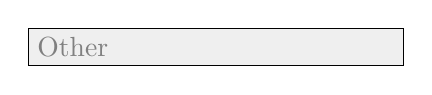
\begin{tikzpicture}
		\node[draw,align=left,fill={rgb:black,1;white,15}] {\color{gray}Other \hspace*{10em}};
	\end{tikzpicture}
}

\newcommand{\longtextfield}{
	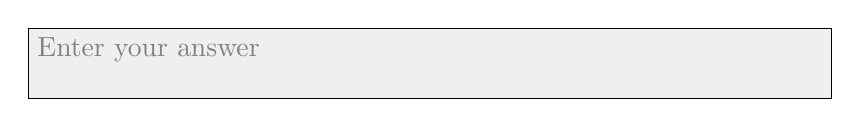
\begin{tikzpicture}
		\node[draw,align=left,fill={rgb:black,1;white,15}] {\color{gray}Enter your answer \hspace*{20em}\\};
	\end{tikzpicture}
}

\newcommand{\likertscaledescription}{
	1\hspace*{2em}2\hspace*{2em}3\hspace*{2em}4\hspace*{2em}5\hspace*{2em}6
}

\newcommand{\likertscalebuttons}{
	\hspace*{0.2em}\radiobutton\hspace*{1.318em}\radiobutton\hspace*{1.318em}\radiobutton\hspace*{1.318em}\radiobutton\hspace*{1.318em}\radiobutton\hspace*{1.318em}\radiobutton\hspace*{0.2em}
}

\newcommand{\likertscalesmall}[2]{
	\begin{center}
		\begin{tabular}{c c c}
			& & \\
			& \likertscaledescription & \\ 
			#1 & \likertscalebuttons & #2 \\
			& & \\
		\end{tabular}
	\end{center}
}

\newcommand{\likertscalelarge}[2]{
	\begin{tabularx}{\textwidth}{X c X}
		& & \\
		& \likertscaledescription & \\ 
		#1 & \likertscalebuttons & #2 \\
		& & \\
	\end{tabularx}
}

This appendix contains the "State of the existing M-Files test automation" survey as it was presented for the M-Files employees. While the survey was first and foremost done to support this thesis, some additional questions were added to the survey to support other M-Files test automation activities. Questions considered in this thesis are marked with a green check mark (\greencheckmark\ ), while questions that are out of the scope of this thesis are marked with the red cross (\redcross\ ). Additionally, an asterisk (\surveyasterix\ ) is used to mark obligatory questions. Even though, from this thesis viewpoint, some questions could have been redacted, all questions were still included for clarity.

\section*{Background}
Little background information about you.

\newlist{question}{enumerate}{1}
\setlist[question,1]{label=\arabic*, leftmargin=*}
\begin{question}
	\item How long have you been working for M-Files?\surveyasterix\greencheckmark
	\begin{itemize}[noitemsep, leftmargin=1.5em]
		\renewcommand\labelitemi{\radiobutton}
		\item Less than a year
		\item 1-2 years
		\item 3-4 years
		\item 5 years or more
	\end{itemize}
	\item What is your current role?\surveyasterix\greencheckmark
	\begin{itemize}[noitemsep, leftmargin=1.5em]
		\renewcommand\labelitemi{\radiobutton}
		\item \gls{qa} engineer
		\item Developer
		\item Product owner
		\item Manager
		\item \othertextfield
	\end{itemize}
	\item What is your current team?\redcross\\
	\begin{surveydescription}
		Note that this question is optional. If you want to retain better anonymity, leave this question unanswered.
	\end{surveydescription}
	\begin{itemize}[noitemsep, leftmargin=1.5em]
		\renewcommand\labelitemi{\radiobutton}
		\item (Exact team names redacted)
		\item \othertextfield
	\end{itemize}
\end{question}

\section*{Test automation-related processes}
This section includes questions about the processes that are related to test automation. This section refers to management processes that guide current test automation activities.

\begin{question}[resume]
	\item Overall, how well are the test automation daily processes working for you?\redcross\\
	\begin{surveydescription}
		Is it effortless to do test automation-related tasks, or is there some extra burden caused by management-related matters?\\
	\end{surveydescription}
	\likertscalesmall{Very poorly}{Very well}
	\item What works well in the current test automation daily processes?\greencheckmark\label{survey_question:works_well_in_processes}\\\\
	\longtextfield
	\item What could be improved in the current test automation daily processes?\greencheckmark\label{survey_question:does_not_work_well_in_processes}\\\\
	\longtextfield
	\item Are you satisfied with the current \gls{dod} related to test automation?\redcross
	\begin{itemize}[noitemsep, leftmargin=1.5em]
		\renewcommand\labelitemi{\radiobutton}
		\item Yes
		\item No
	\end{itemize}
	\item How current test automation \gls{dod} could be improved\greencheckmark\label{survey_question:how_dod_can_be_improved}\\\\
	\longtextfield
\end{question}

\section*{Test automation feelings \& attitudes}
These questions measure your current feelings and attitudes towards test automation and chart the reasons behind the measures.

\begin{question}[resume]
	\item After making code changes, how much confidence test automation provides for you that your changes will not break something else unexpectedly?\redcross\\
	\likertscalelarge{Test automation doesn't give me any confidence}{I'm assured that my changes won't break anything}
	\item Please elaborate further, why the current test automation provides or doesn't provide confidence for you?\greencheckmark\label{survey_question:test_automation_confidence}\\\\
	\longtextfield
	\item Does the current test automation produce value for you?\redcross\\
	\likertscalelarge{Test automation hinders my daily work}{Test automation is extremely useful for me}
	\item Please elaborate further, why the current test automation provides or doesn't provide value for you?\greencheckmark\label{survey_question:test_automation_value}\\\\
	\longtextfield
	\item When automated test case fails while developing a user story, what do you commonly do?\redcross
	\begin{itemize}[noitemsep, leftmargin=1.5em]
		\renewcommand\labelitemi{\radiobutton}
		\item I check the failure, fix the code if necessary and rerun.
		\item I rerun the pipeline once again and then check the errors to see if they are still persisting.
		\item I rerun the pipeline multiple times without checking the errors.
		\item I contact the test automation team after the failure.
		\item \othertextfield
	\end{itemize}
	\item When implementing a user story, do you consider creating new test automation cases?\redcross
	\begin{itemize}[noitemsep, leftmargin=1.5em]
		\renewcommand\labelitemi{\radiobutton}
		\item Always
		\item Often
		\item Sometimes
		\item Never
		\item \othertextfield
	\end{itemize}
	\item Please elaborate further on why you have or don't have a good attitude towards test automation?\greencheckmark\label{survey_question:test_automation_attitude}\\\\
	\longtextfield
\end{question}

\section*{Knowledge and education-related questions}
During the section, it is measured how much you know about the current test automation and how you would like to increase your knowledge about it.

\begin{question}[resume]
	\item Do you think you have sufficient knowledge to do test automation cases?\greencheckmark\label{survey_question:sufficient_test_automation_knowledge}
	\begin{itemize}[noitemsep, leftmargin=1.5em]
		\renewcommand\labelitemi{\radiobutton}
		\item Yes
		\item No
		\item \othertextfield
	\end{itemize}
	\item Overall, how would you describe your M-Files test automation knowledge?\redcross
	\begin{itemize}[noitemsep, leftmargin=1.5em]
		\renewcommand\labelitemi{\radiobutton}
		\item Never heard
		\item Heard but never interacted with it
		\item Executed pipelines, but I will be in trouble if anything breaks
		\item I'm able to investigate failures
		\item I have created my own test cases
		\item I'm able to teach others
		\item \othertextfield
	\end{itemize}
	\item How much do you know about the following subjects?\redcross
	\begin{center}
		\rowcolors{1}{rgb:black,1;white,30}{}
		\begin{tabularx}{\textwidth}{X c c c c c c}
			\rowcolor{rgb:white,1} & &  & Less than & More than & Quite & \\
			& Nothing & Something & average & average & much & Everything\\
			M-Files integration testing & \radiobutton & \radiobutton & \radiobutton & \radiobutton & \radiobutton & \radiobutton\\
			Quality assurance in general & \radiobutton & \radiobutton & \radiobutton & \radiobutton & \radiobutton & \radiobutton\\
			vNext UI test automation & \radiobutton & \radiobutton & \radiobutton & \radiobutton & \radiobutton & \radiobutton\\
			Usage of the TeamCity & \radiobutton & \radiobutton & \radiobutton & \radiobutton & \radiobutton & \radiobutton\\
			Testing in general & \radiobutton & \radiobutton & \radiobutton & \radiobutton & \radiobutton & \radiobutton\\
			M-Files unit testing & \radiobutton & \radiobutton & \radiobutton & \radiobutton & \radiobutton & \radiobutton\\
			Test automation processes & \radiobutton & \radiobutton & \radiobutton & \radiobutton & \radiobutton & \radiobutton\\
			Usage of the test automation pipelines & \radiobutton & \radiobutton & \radiobutton & \radiobutton & \radiobutton & \radiobutton\\
			Test automation in general & \radiobutton & \radiobutton & \radiobutton & \radiobutton & \radiobutton & \radiobutton\\
		\end{tabularx}
	\end{center}
	\item If some test automation-related aspects aren't familiar to you, which aspects would you like to know more about?\redcross
	\begin{itemize}[noitemsep, leftmargin=1.5em]
		\renewcommand\labelitemi{$\square$}
		\item Quality assurance
		\item Testing in general
		\item Test automation in general
		\item Test automation processes
		\item Usage of the TeamCity
		\item M-Files unit testing
		\item M-Files integration testing
		\item vNext UI test automation
		\item \othertextfield
	\end{itemize}
	\item Which way would you like to learn more about test automation?\greencheckmark\label{survey_question:preferred_ways_of_learning}
	\begin{itemize}[noitemsep, leftmargin=1.5em]
		\renewcommand\labelitemi{$\square$}
		\item Test automation champions for teams
		\item Better documentation
		\item Training sessions
		\item Test automation workshops
		\item Tutoring
		\item \othertextfield
	\end{itemize}
\end{question}

\section*{Technical details}
In this section, you can give feedback about the current technical details of the test automation systems.

\begin{question}[resume]
	\item How important following test automation aspects are for you?\greencheckmark\label{survey_question:importance_of_test_automation_ascpects}
	\begin{center}
		\rowcolors{1}{}{rgb:black,1;white,30}
		\begin{tabularx}{\textwidth}{X c c c c c c}
			\rowcolor{rgb:white,1} &  &  & Not &  &  & \\
			\rowcolor{rgb:white,1} & & Not & especially & Somewhat & Very & \\
			\rowcolor{rgb:white,1} & Indifferent & Important & important & important & Important & important \\
			Execution speed & \radiobutton & \radiobutton & \radiobutton & \radiobutton & \radiobutton & \radiobutton\\
			Reliability & \radiobutton & \radiobutton & \radiobutton & \radiobutton & \radiobutton & \radiobutton\\
			Clear error messages & \radiobutton & \radiobutton & \radiobutton & \radiobutton & \radiobutton & \radiobutton\\
			Ease of development environment setup & \radiobutton & \radiobutton & \radiobutton & \radiobutton & \radiobutton & \radiobutton\\
			Ease of development & \radiobutton & \radiobutton & \radiobutton & \radiobutton & \radiobutton & \radiobutton\\
		\end{tabularx}
	\end{center}
	\item What is good in the current M-Files unit test automation systems?\greencheckmark\label{survey_question:good_in_unit_test_automation}\\
	\begin{surveydescription}
		Is the test automation easy to set up, fast, and pleasant to use... Please note that you may provide comments regarding any unit test automation systems.
	\end{surveydescription}
	\longtextfield
	\item What doesn't work in the current M-Files unit test automation systems?\greencheckmark\\
	\begin{surveydescription}
		Is there something that just doesn't click? Please note that you may provide comments regarding any unit test automation systems.
	\end{surveydescription}
	\longtextfield
	\item Please specify which unit test automation systems your above answers refer to.\greencheckmark
	\begin{itemize}[noitemsep, leftmargin=1.5em]
		\renewcommand\labelitemi{$\square$}
		\item M-Files core C++
		\item M-Files core C\#
		\item \othertextfield
	\end{itemize}
	\item What is good in the current M-Files integration test automation systems?\greencheckmark\label{survey_question:good_in_integration_test_automation}\\
	\begin{surveydescription}
		Is the test automation easy to set up, fast, and pleasant to use... Please note that you may provide comments regarding any integration test automation systems.
	\end{surveydescription}
	\longtextfield
	\item What doesn't work in the current M-Files integration test automation systems?\greencheckmark\\
	\begin{surveydescription}
		Is there something that just doesn't click? Please note that you may provide comments regarding any integration test automation system.
	\end{surveydescription}
	\longtextfield
	\item Please specify which integration test automation systems your above answers refer to.\greencheckmark
	\begin{itemize}[noitemsep, leftmargin=1.5em]
		\renewcommand\labelitemi{$\square$}
		\item M-Files core integration tests
		\item \othertextfield
	\end{itemize}
	\item What is good in the current M-Files \gls{ui} test automation systems?\greencheckmark\label{survey_question:good_in_ui_test_automation}\\
	\begin{surveydescription}
		Is the test automation easy to set up, fast, and pleasant to use... Please note that you may provide comments regarding any \gls{ui} test automation systems.
	\end{surveydescription}
	\longtextfield
	\item What doesn't work in the current M-Files \gls{ui} test automation systems?\greencheckmark\\
	\begin{surveydescription}
		Is there something that just doesn't click? Please note that you may provide comments regarding any \gls{ui} test automation system.
	\end{surveydescription}
	\longtextfield
	\item Please specify which \gls{ui} test automation systems your above answers refer to.\greencheckmark
	\begin{itemize}[noitemsep, leftmargin=1.5em]
		\renewcommand\labelitemi{$\square$}
		\item vNext test automation
		\item M-Files desktop test automation
		\item \othertextfield
	\end{itemize}
	\item What is good in the current M-Files test automation pipelines?\greencheckmark\label{survey_question:good_in_pipelines}\\
	\begin{surveydescription}
		Are pipelines easy to use, clear, fast... Please note that you may provide comments regarding any M-Files pipelines.
	\end{surveydescription}
	\longtextfield
	\item What doesn't work in the current M-Files test automation pipelines?\greencheckmark\\
	\begin{surveydescription}
		Is there something that just doesn't click? Please note that you may provide comments regarding any M-Files pipelines.
	\end{surveydescription}
	\longtextfield
	\item Please specify, which test automation pipelines your above answers refers to.\greencheckmark
	\begin{itemize}[noitemsep, leftmargin=1.5em]
		\renewcommand\labelitemi{$\square$}
		\item M-Files core pipelines
		\item vNext pipelines
		\item \othertextfield
	\end{itemize}
\end{question}

\section*{Final thoughts}
In this section, you can provide final thoughts about the test automation and give free-form feedback.

\begin{question}[resume]
	\item Overall, how satisfied are you with the current M-Files test automation?\surveyasterix\redcross\\\\
	\huge\ding{73} \ding{73} \ding{73} \ding{73} \ding{73}\normalsize
	\item Any other thoughts about the test automation?\greencheckmark\\\\
	\longtextfield
\end{question}